\documentclass{article}

\newenvironment{nscenter}
  {\parskip=0pt\par\nopagebreak\centering}
  {\par\noindent\ignorespacesafterend}

\usepackage{wrapfig}
\usepackage{amsmath}
\usepackage{mdframed}

\mdfdefinestyle{MyFrame}{%
  linecolor=black,
  outerlinewidth=2pt,
  %roundcorner=20pt,
  innertopmargin=4pt,
  innerbottommargin=4pt,
  innerrightmargin=4pt,
  innerleftmargin=4pt,
  leftmargin = 4pt,
  rightmargin = 4pt
  %backgroundcolor=gray!50!white}
}

\usepackage{ulem}
\usepackage{tikz}
\usepackage{fullpage}
\usepackage{graphicx}
\usepackage{subcaption}
% Table Formatting
\usepackage{multirow}
\usepackage{booktabs}
\usepackage{longtable}
\usepackage{siunitx}

\sisetup{
  round-mode          = places, % Rounds numbers
  round-precision     = 2, % to 2 places
}

% \setlength{\parskip}{\baselineskip}%
\setlength{\parindent}{0pt}

\title{University Physics I - PHYS 1211}
\date{July 13, 2024}
\author{Ethan Anthony}

\begin{document}
\pagenumbering{arabic}
\maketitle
\tableofcontents
\newpage

\section{Conceptual Introduction}
\subsection{Reference Frames}
\textbf{A reference frame} is the context in which a quantities and processes are described.
It defines the absolute baseline that properties such as position and velocity are relative to.
The position of an object at a given point of time is absolute. It exists in a single,
absolute, point in space. However, rather that only being able to describe its position in
absolute terms, one can create a reference frame to describe its position in more local, and
more meaningful, terms.

\begin{center}
  % \includegraphics[width=\linewidth]{figures/figure.png}
\end{center}

Here we have three points on a line. Nowhere is it defined where these points are in
absolute space. However, in reference to the number line, the red point is at $0$, 
the green point is at $-1$ and the blue point is at $2$.

\begin{center}
  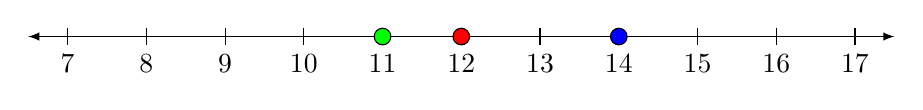
\begin{tikzpicture}
    \draw[latex-latex] (-5.5,0) -- (5.5,0) ;
    \foreach \x in  {-5, -4, -3, -2, -1, 0, 1, 2, 3, 4, 5}
    \draw[shift={(\x,0)},color=black] (0pt,3pt) -- (0pt,-3pt);
    \foreach \x in  {-5, -4, -3, -2, -1, 0, 1, 2, 3, 4, 5}
    \draw[shift={(\x,0)},color=black] (0pt,0pt) -- (0pt,-3pt) node[below] 
      {\the\numexpr\x + 12\relax};
    \draw[fill=red] (0,0) circle (3pt) ;
    \draw[fill=green] (-1,0) circle (3pt) ;
    \draw[fill=blue] (2,0) circle (3pt) ;
  \end{tikzpicture}
\end{center}

Here, the points themselves have not moved, but rather than being the red point, green point, 
and blue point being in positions $0$, $-1$, and $2$ respctively, they are now
in positions $12$, $11$, and $14$. This is due to the \textit{reference frame} changing, 
not the positions of the points.

\subsection{Position and Displacement}
\textbf{Position} describes an objects location in space, relative to its reference frame.
In the examples above, the reference frame defined a range of numbers corresponding to different
points in space, and the position of each point was where it was relative to those defined
numbers.
\\[12pt]
\textbf{Displacement} is a net change in position. Consider the path the point takes below.
The point starts at $0$, then moves to $-4$, then moves to $3$ where it stops. 

\begin{center}
  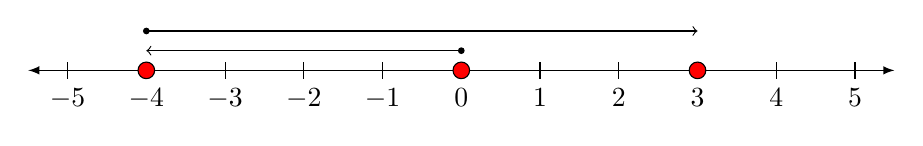
\begin{tikzpicture}
    \draw[latex-latex] (-5.5,0) -- (5.5,0) ;
    \foreach \x in  {-5, -4, -3, -2, -1, 0, 1, 2, 3, 4, 5}
    \draw[shift={(\x,0)},color=black] (0pt,3pt) -- (0pt,-3pt);
    \foreach \x in  {-5, -4, -3, -2, -1, 0, 1, 2, 3, 4, 5}
    \draw[shift={(\x,0)},color=black] (0pt,0pt) -- (0pt,-3pt) node[below] 
      {$\x$};
    \draw[fill=red] (0,0) circle (3pt) ;
    \draw[fill=red] (-4,0) circle (3pt) ;
    \draw[fill=red] (3,0) circle (3pt) ;
    \draw[->] (0,0.25) -- (-4,0.25) ;
    \draw[fill=black] (0,0.25) circle (1pt) ;
    \draw[->] (-4,0.5) -- (3,0.5) ;
    \draw[fill=black] (-4, 0.5) circle (1pt) ;
  \end{tikzpicture}
\end{center}

Though it moved first to $-4$ before arriving at $3$, its displacement is still only $3$. This can be calculated
in two different ways First is to add up each movement: $-4+7=3$. Second is to subtract
its initial position from its final position: $3-0=3$. As can be seen, both lead to the same
answer of a displacement on $3$. The simpler of the two is the second method, which is expressed
as follows:

\begin{equation} \label{Displacement Equation}
  \begin{split}
    \textup{Displacement} & = \textup{Final Position} - \textup{Initial Position} \\
    \Delta x & = x_{final} - x_{initial}
  \end{split}
\end{equation}

\subsection{Position as a Function of Time}

\begin{wrapfigure}{R}{8cm}
  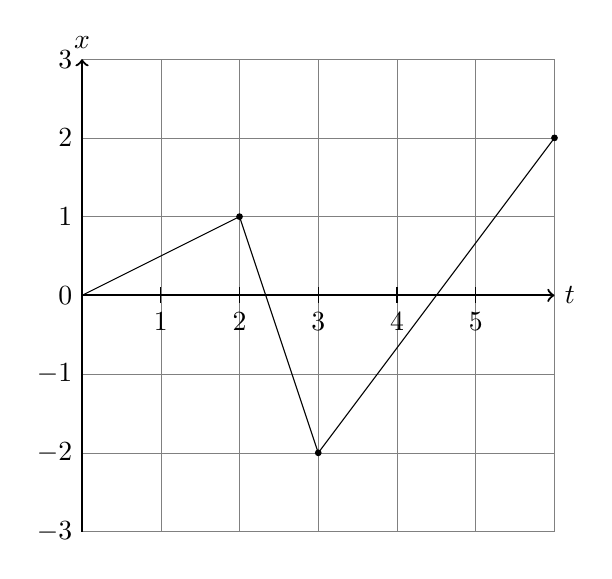
\begin{tikzpicture}
    \draw[help lines] (0,0) grid (6,6) ;
    \draw[->, thick] (0,3) -- (6,3) node[right] {$t$} ;
    \draw[->, thick] (0,0) -- (0,6) node[above] {$x$} ;
    \foreach \x in {1, 2, 3, 4, 5}
    \draw[shift={(\x,0)}] (0pt,3.1) -- (0pt,2.9) node[below] {$\x$} ;
    \foreach \x in {-3, -2, -1, 0, 1, 2, 3}
    \draw[shift={(0, \x)}] (0,3) node[left] {$\x$} ;
    \draw[] (0,3) -- (2,4) ;
    \draw[fill=black] (2,4) circle (1pt) ;
    \draw[] (2,4) -- (3,1) ;
    \draw[fill=black] (3,1) circle (1pt) ;
    \draw[] (3,1) -- (6,5) ;
    \draw[fill=black] (6,5) circle (1pt) ;
  \end{tikzpicture}
  \caption{Position vs. Time}
\end{wrapfigure}

Objects' movement happen in time. For an object to go from one place to another, some amount
of time must pass. \textit{Figure 1} is a \textbf{Position vs. Time Graph}. On the
horizontal axis is time ($t$). On the vertical axis is an object's position ($x$). In the 
first two units of time, the object moves from position $0$ to position $1$. From there it
moves to position $-2$ in one unit of time, and finally arrives at position $2$ in three 
additional units of time. Using this example, displacement can be calculated with our displacement
equation. 
\begin{equation*}
  \Delta x = x_{final} - x_{initial} \Rightarrow \Delta x = x_{6} - x_{0} \Rightarrow \Delta x = 2 - 0 \Rightarrow \Delta x = 2
\end{equation*}

\textbf{Speed} is a measurement of how fast something is moving over time. It is a scalar
quantity, meaning that it has a magnitude, but no direction. It can be expressed
as $\frac{\Delta x_{net}}{\Delta t}$, which is the distance traveled divided by the time taken
to travel that distance. Distance traveled has no positive or negative, it is a absolute measurement.
In \textit{Figure 1}, over the inverval $0<t<2$, the distance traveled is $1$. Similarly, it
is $3$ over $2<t<3$ and $4$ over $3<t<6$. In total, a distance of $8$ is traveled. Using our
equation for speed:
\begin{equation*}
  \textup{Speed} = \frac{\Delta x_{net}}{\Delta t} = \frac{8}{6} = 1.33
\end{equation*}
\textbf{Velocity} is also a measurement of how fast something is moving over time, but rather
than being a scalar quantity, it is a vector. This means that it measures both direction \textit{and}
magnitude. It can be expressed as $\frac{\Delta x}{\Delta t}$; displacement over time. Using
the same quantities as previous, we can calculate the velocity of the object in \textit{Figure 1}
as:
\begin{equation*}
  v = \frac{\Delta x}{\Delta t} = \frac{2}{6} = 0.33
\end{equation*}
This not only tells us that the speed at which the object was moving was 0.33, but also that 
it was moving in the positive direction over the interval $0<t<6$.

\subsection{Units of Measurement}
\begin{wrapfigure}{L}{10cm}
  \begin{nscenter}
    \caption{SI Base Units}
    \begin{tabular}{l|c|r}
      \toprule
      \textbf{Quantity} & \textbf{Name} & \textbf{Symbol} \\
      \midrule
      Length                    & meter    & $m$   \\
      Mass                      & kilogram & $kg$  \\
      Time                      & second   & $s$   \\
      Current                   & ampere   & $A$   \\
      Thermodynamic Temperature & kelvin   & $K$   \\
      Amount of Substance       & mole     & $mol$ \\
      Luminous Intensity        & candela  & $cd$  \\
      \bottomrule
    \end{tabular}
  \end{nscenter}
\end{wrapfigure}

Thusfar, we have been speaking only in terms of values, but not of concrete units. When we
said that the object was moving with a velocity of $0.33$, or that it had a position of $-3$,
these numbers were abstract; they had no concrete meaning behind them. In physics, there is 
a standard set of units that are used: the \textbf{SI Units}. There are countless SI Units, 
however, only seven \textbf{SI Base Units}, the units which every other unit is derived from. 
For example, length ($m$) and time ($s$) both are base units, but velocity ($\frac{m}{s}$)
is a unit \textit{composed of} two base units. Using this, we can say that the position of a
point is at $-3m$ or the velocity of that object is $0.33 \frac{m}{s}$.

\subsection{Instentaneous Velocity}
\textbf{Instentaneous velocity} is the rate at which an object is moving at a \textit{single point of time}.
Previously, we defined velocity as $\frac{\Delta x}{\Delta t}$. In reality, this was \textit{average}
velocity. As seen in \textit{Figure 3}, the red dotted line represents the average velocity over the 
period of time of $0<t<10$. The blue line, however, represents the instentaneous velocity
of the object at $t=6$. This line runs tangent (intersects at a single point) to the position function,
thus the slope of the tangent line is the instentaneous velocity where it intersects ($t=6$).

\begin{wrapfigure}{L}{7cm}
  \begin{center}
    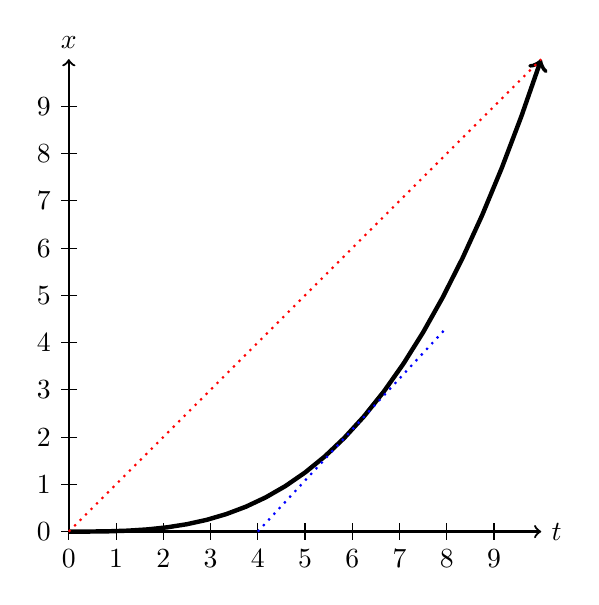
\begin{tikzpicture}[scale=6]
      \draw[->, thick] (0,0) -- (1,0) node[right] {$t$} ;
      \draw[->, thick] (0,0) -- (0,1) node[above] {$x$} ;
      \foreach \x in {0, 1, 2, 3, 4, 5, 6, 7, 8, 9}
      \draw[shift={({\x/10},0)}] (0pt,0.5pt) -- (0pt,-0.5pt) node[below] {$\x$} ;
      \foreach \x in {0, 1, 2, 3, 4, 5, 6, 7, 8, 9}
      \draw[shift={(0,{\x/10})}] (0.5pt,0pt) -- (-0.5pt,0pt) node[left] {$\x$} ;
      \draw[ultra thick, black, ->, domain=0:1] plot ({\x, \x*\x*\x}) ;
      \draw[thick, dotted, red, domain=0:1] plot ({\x, \x}) ;
      \draw[thick, dotted, blue, domain=0.4:0.8] plot ({\x, {(1.08*\x)-0.432}}) ;
    \end{tikzpicture}
    \caption{Instentaneous vs. Average Velocity}
  \end{center}
\end{wrapfigure}



\end{document}
